\begin{enumerate}[label=\thesubsection.\arabic*,ref=\thesubsection.\theenumi]
\item Find the slope of the tangent to the curve $y = \frac{x-1}{x-2}$, $x \neq 2$ at $x=10$.
	\\
\solution 
\label{chapters/12/6/3/2}
The given equation of the curve can be rearranged as
\begin{align}
	xy-x-2y+1 &= 0 \\
        \label{eq:chapters/12/6/3/2/Eq1}
	\implies \vec{x}^\top\myvec{0 & \frac{1}{2} \\ \frac{1}{2} & 0}\vec{x} + \myvec{-1 & -2}\vec{x}+1 &= 0 
\end{align}
Thus, 
\begin{align}
	\vec{V} &= \myvec{ 0 & \frac{1}{2} \\ \frac{1}{2} & 0} \\
	\vec{u} &= -\myvec{\frac{1}{2} \\ 1} \\
	f &= 1 
\end{align}
$\because q_1 = 10$, the point of contact can be obtained as
\begin{align}
	 \vec{q} =\myvec{q_1 \\ q_2} = \myvec{10 \\ \frac{9}{8}}
\end{align}
  From \eqref{eq:conic_tangent_mq},
 the normal vector of the tangent to \eqref{eq:chapters/12/6/3/2/Eq1} is
\begin{align}
	\vec{n} = \myvec{1 \\ 64}
	\implies
	\vec{m} = \myvec{1 \\ \frac{-1}{64}}
\end{align}
The eigenvector matrix 
\begin{align}
	\myvec{\vec{p}_1 & \vec{p}_2} = \frac{1}{\sqrt{2}}\myvec{1 & 1 \\ 1 & -1}
\end{align}
which implies that  the conic is a $45\degree$ rotated hyperbola.
See \figref{fig:chapters/12/6/3/2/Fig1}.
\begin{figure}[H]
	\begin{center}
		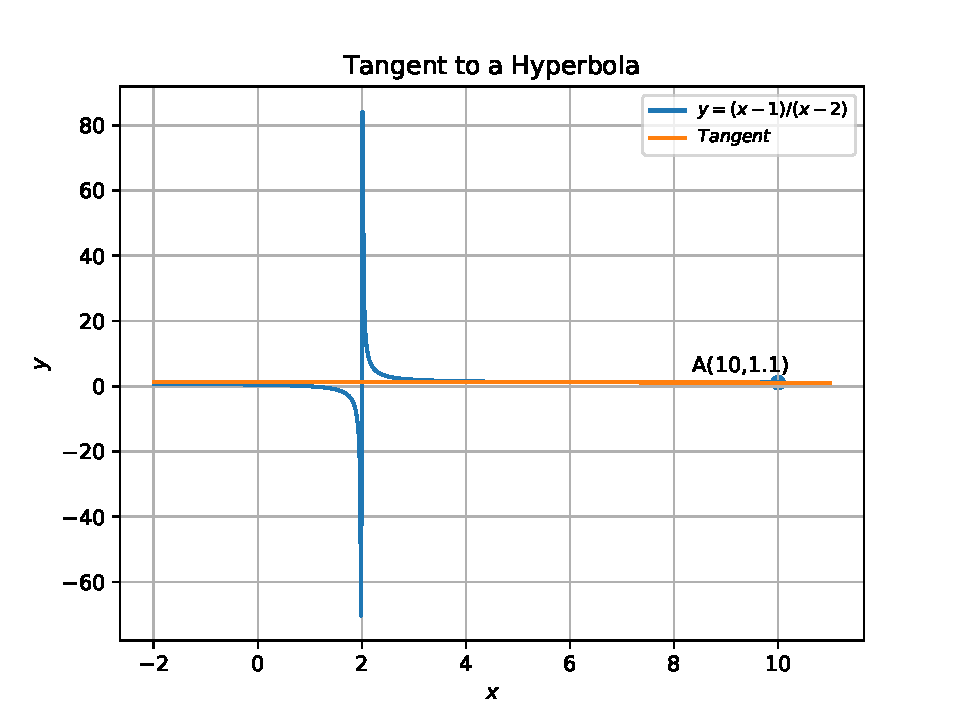
\includegraphics[width=0.75\columnwidth]{chapters/12/6/3/2/figs/problem2.pdf}
	\end{center}
\caption{}
\label{fig:chapters/12/6/3/2/Fig1}
\end{figure}

\item 
		Find a point on the curve \begin{align}y=(x-2)^2\end{align} at which a tangent is parallel to the chord joining the points (2,0) and (4,4).
			\\
			\solution 
\label{chapters/12/6/3/8}
	\begin{figure}[!ht]
		\centering
 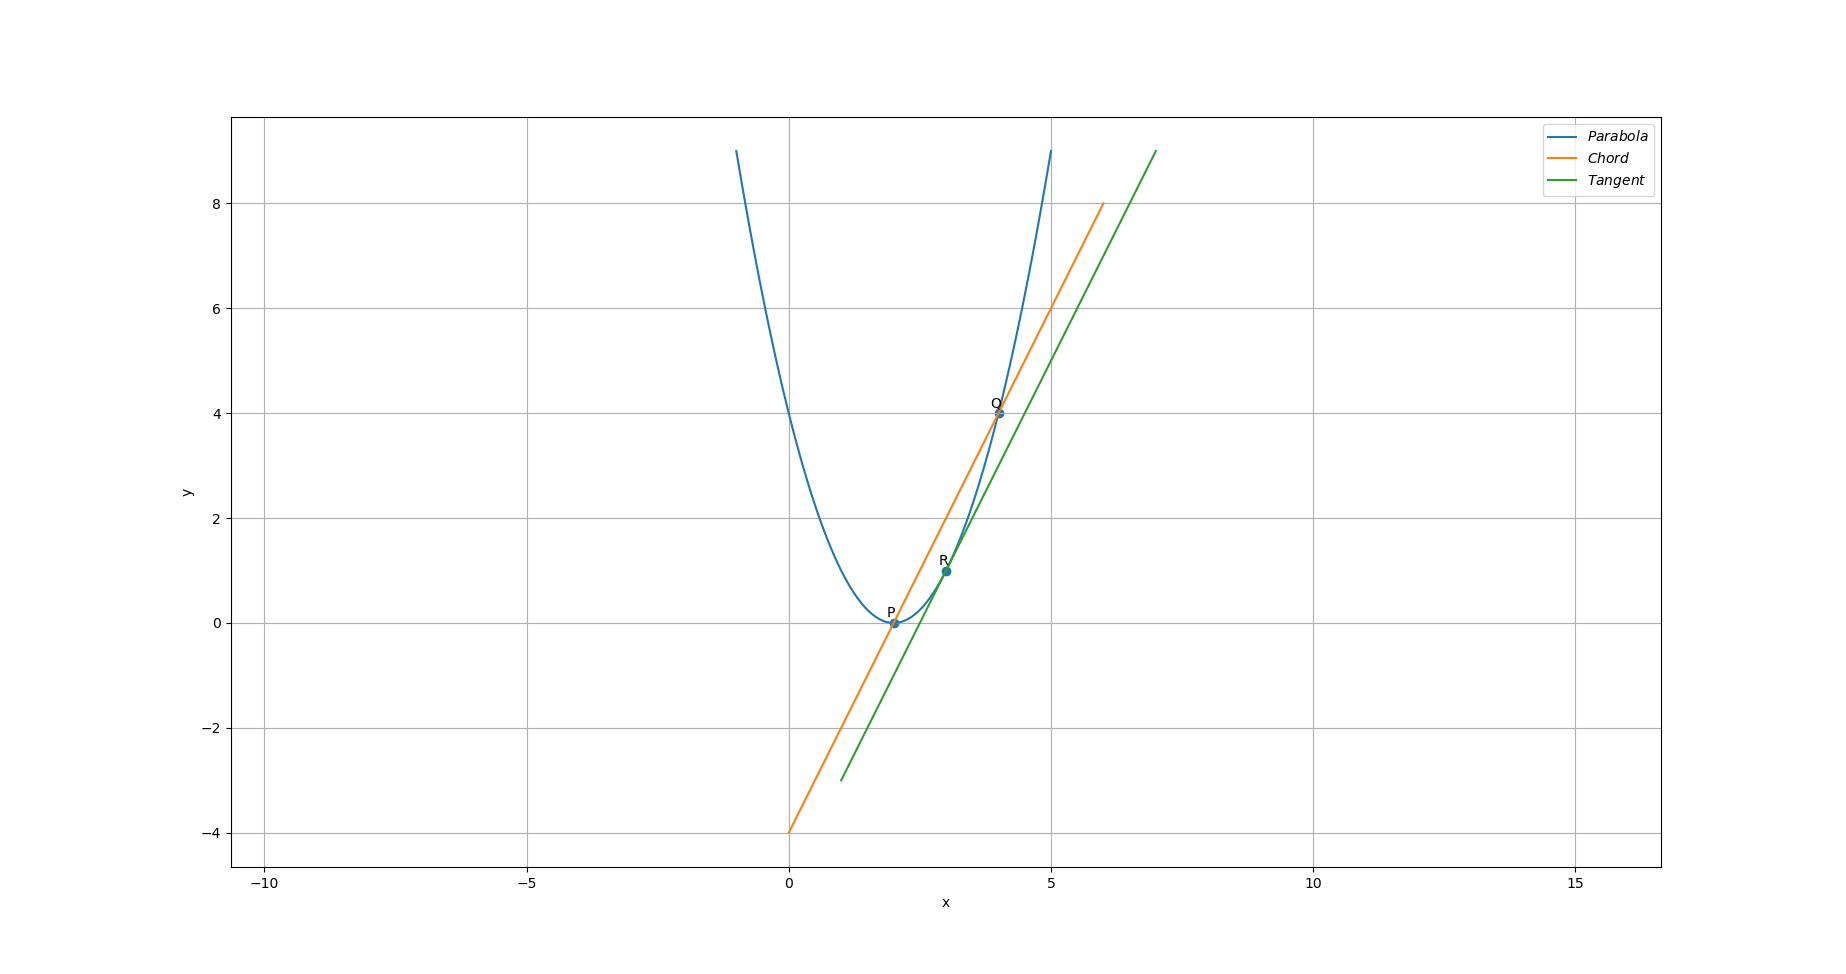
\includegraphics[width=\columnwidth]{chapters/12/6/3/8/figs/main.png}
		\caption{}
		\label{fig:12/6/3/8}
  	\end{figure}
The equation of the conic can be represented as
\begin{align}
\vec{x}^{\top}\myvec{1&0\\0&0}\vec{x}+2\myvec{-2&\frac{-1}{2}}\vec{x}+4=0
\end{align}
So,
\begin{align}
\vec{V}=\myvec{1&0\\0&0},
\vec{u}^{\top}=\myvec{-2&\frac{-1}{2}},
f=4
\end{align}
The direction vector of the line passing through (2,0) and (4,4) is 
\begin{align}
\vec{m}=\myvec{1\\2}
\implies
\vec{n}=\myvec{2\\-1}.
\end{align}
The eigenvector corresponding to the zero eigenvalue is 
\begin{align}
\vec{p}_1=\myvec{0\\1},
\end{align}
In
\eqref{eq:conic_tangent_q_eigen},
\begin{align}
	\kappa=\frac{\myvec{0&1}\myvec{-2\\ \frac{-1}{2}}}{\myvec{0&1}\myvec{2\\-1}}
	=\frac{1}{2}
\end{align}
Substituting  $\kappa$,
from 
\eqref{eq:conic_tangent_q_eigen},
\begin{align}
	\myvec{\sbrak{\myvec{-2\\\frac{-1}{2}}+\frac{1}{2}\myvec{2\\-1}}^{\top} \\ \myvec{1&0\\0&0}}\vec{q} &= \myvec{-4 \\ \frac{1}{2}\myvec{2\\-1}-\myvec{-2\\\frac{-1}{2}}}\\
	\implies
	\myvec{-1&-1 \\ 1&0 \\ 0&0}\vec{q}&=\myvec{-4 \\ 3 \\ 0}
\end{align}
yielding
\begin{align}
\myvec{-1&-1 \\ 1&0}\vec{q} = \myvec{-4\\3}
\end{align}
The augmented matrix is 
\begin{align*}
  \myvec{
                -1&-1&\vrule&-4\\
	        1&0&\vrule&3}
  \xleftrightarrow[]{R_1 \leftarrow R_1+ 2R_2}
     \myvec{
	         1&-1&\vrule&2\\
	         1&0&\vrule&3}
      \\
 \xleftrightarrow[]{R_2 \leftarrow R_2 - R_1}
     \myvec{
	         1&-1&\vrule&2\\
	         0&1&\vrule&1}
 \xleftrightarrow[]{R_1 \leftarrow R_1 + R_2}
     \myvec{
	         1&0&\vrule&3\\
	         0&1&\vrule&1}
      \\ \implies \vec{q}=\myvec{3\\1}
\end{align*}
which is the desired 
point of contact.
See Fig. 
		\ref{fig:12/6/3/8}.

\item 
Find the equation of all lines having slope  -1 that are tangents to the curve
\begin{align}
y = \frac{1}{x-1}, x \neq 1
\label{chapters/12/6/3/10}
\end{align}
	\\
	\solution 
\iffalse
\documentclass{article}
% Language setting
% Replace `english' with e.g. `spanish' to change the document language
\usepackage[english]{babel}
% Set page size and margins
% Replace `letterpaper' with `a4paper' for UK/EU standard size
\usepackage[letterpaper,top=2cm,bottom=2cm,left=3cm,right=3cm,marginparwidth=1.75cm]{geometry}
% Useful packages
\usepackage{multicol}
\usepackage{amsmath}
\usepackage{amssymb}
\usepackage{graphicx}
\usepackage[framemethod=tikz]{mdframed}
\usepackage{array}
\usepackage{blindtext}
%\usepackage[paperwidth=10cm]{geometry}
\usepackage{tkz-euclide}
%\usepackage{tikz}
\usetikzlibrary{
  circuits.logic,
  circuits.logic.US,
  positioning
}

\usepackage[colorlinks=true, allcolors=blue]{hyperref}
\newcommand{\myvec}[1]{\ensuremath{\myvec{#1}}}
\providecommand{\norm}[1]{\left\lVert#1\right\rVert}
\let\vec\mathbf
\title{Conic Assignment}
\author{Anusha Jella}
\begin{document}
\maketitle
\newtheorem{theorem}{Theorem}[section]
\begin{multicols}{2}

\paragraph{\begin{flushleft}\textbf{Problem: }
	\fi
Find the equation of all lines having slope  -1 that are tangents to the curve
\begin{align}
y = \frac{1}{x-1}, x \neq 1
\end{align}
	\begin{figure}[!ht]
		\centering
 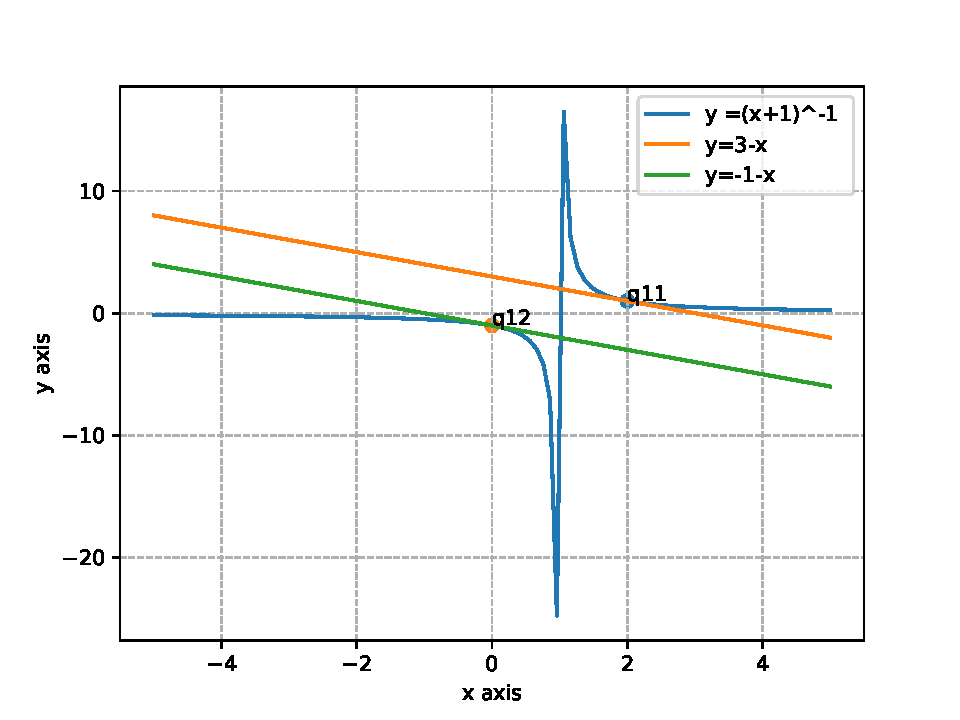
\includegraphics[width=\columnwidth]{chapters/12/6/3/10/figs/conic1.pdf}
		\caption{}
		\label{fig:12/6/3/10}
  	\end{figure}
	\\
	\solution 
\iffalse
\end{flushleft}}
%\begin{figure}[h]
\centering
\includegraphics[scale=0.5]{conic_fig1.pdf} 
%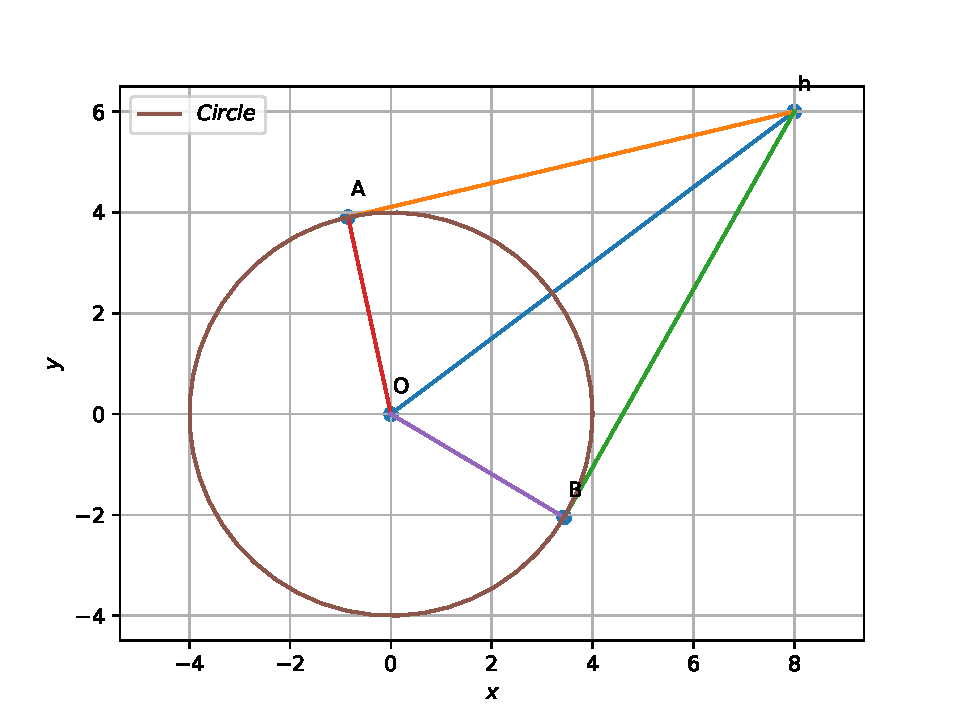
\includegraphics[width=\columnwidth]{circle1.pdf} 
\centering{Fig 1. Curve}
\label{fig:circle_1}
%\end{figure}

 \section*{Construction}
 \begin{flushleft}
 \textsc{solution:} The following python code is used for constructing conic with tangents.
 \end{flushleft}
 \begin{mdframed}
   \url{https://github.com/AnushaJella/assignment_conic/blob/main/conic1.py}\\
\end{mdframed}
See Fig 1 for the input parameters in Table 1.\\
\vspace{0.5cm}
{\setlength\extrarowheight{2pt}
\begin{tabular}{|c|c|c|}
	\hline
	\textbf{Symbol}&\textbf{Value}&\textbf{Description}\\
	\hline
	$\textbf{x}$&[-5,5,100] &to find $\textbf{y}$\\
	\hline
\end{tabular}
}\\
\centering {Table 1}\\
\section*{Solution}
\begin{flushleft}
The equation of  a conic with directrix $\vec{n}^{\top}\vec{x} = c$, eccentricity $e$ and focus $\vec{F}$ is given by 
\end{flushleft}
\begin{align}
    \vec{x}^{\top}\vec{V}\vec{x}+2\vec{u}^{\top}\vec{x}+f=0
    \end{align}
\hspace{-6.5cm}where     
\begin{align}
  \label{eq:conic_quad_form_v}
\vec{V} &=\norm{\vec{n}}^2\vec{I}-e^2\vec{n}\vec{n}^{\top}, 
\\
\label{eq:conic_quad_form_u}
\vec{u} &= ce^2\vec{n}-\norm{\vec{n}}^2\vec{F}, 
\\
  f &= \norm{\vec{n}}^2\norm{\vec{F}}^2-c^2e^2
\end{align}
\hspace{-6.5cm}Given, 
\fi
From the given information, 
\begin{align}
	\vec{V}
	=\myvec{
		0 & \frac{1}{2}\\\frac{1}{2}& 0\\
	},
\vec{u} = \myvec{
0 \\-\frac{1}{2}\\
},  f = -1, m=-1
	\label{eq:matrix-10-13-param}
\end{align}
From the above, the  normal vector is
\begin{align}
\vec{n}=\myvec{
-m \\ 1
	} = \myvec{1 \\ 1}
	\label{eq:matrix-10-13-param-n}
\end{align}
From 
\eqref{eq:conic_tangent_qk},
	the point(s) of contact are given by
\begin{align}
	\vec{q}&=\vec{V}^{-1}(k_i\vec{n}-\vec{u}) 
	\text{ where},\\
	k_i&=\pm \sqrt{\frac{f_0}{\vec{n}^{\top}\vec{V}^{-1}\vec{n}}}\\
	f_0&=f+\vec{u}^{\top}\vec{V}^{-1}\vec{u}
\end{align}
Substituting from 
	\eqref{eq:matrix-10-13-param-n}
	and
	\eqref{eq:matrix-10-13-param}
	in the above,
\begin{align}
\vec{q}=\myvec{0 \\-1}, \myvec{2 \\ 1}.
\end{align}
From 
  \eqref{eq:conic_tangent_final},
the equations of tangents are given by
\begin{align}
(\vec{V}\vec{q}+\vec{u})^{\top}\vec{x}+\vec{u}^{\top}\vec{q}+f=0
\end{align}
yielding
\begin{align}
	\myvec{1 & 1}\vec{x}+1&=0\\
\myvec{1 & 1}\vec{x}-3&=0\\
\end{align}
See Fig. 
		\ref{fig:12/6/3/10}.
\iffalse

\end{multicols}{2}
\end{document}
\fi

\item 
Find the equation of all lines having slope 2 which are tangents to the curve 
\begin{align}
y=\frac{1}{x-3}, x\neq{3} 
\end{align}
\solution 
\label{chapters/12/6/3/11}
	\begin{figure}[!ht]
		\centering
 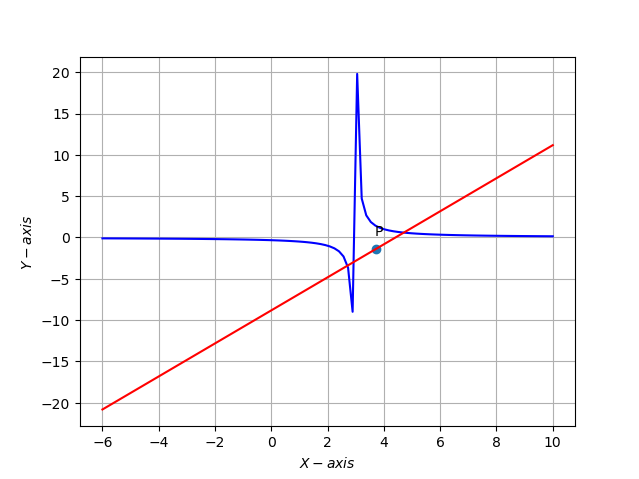
\includegraphics[width=\columnwidth]{chapters/12/6/3/11/figs/con_fig.png}
		\caption{}
		\label{fig:12/6/3/11}
  	\end{figure}
From the given information
\begin{align}
	\vec{V}
	&=\myvec{
		0 &\frac{1}{2}\\\frac{1}{2} & 0\\
	},
\vec{u} = \myvec{
0 \\-\frac{3}{2}
},  f = -1, m=2
	\label{12/6/3/11/eq1}
	\\
	\implies
	\vec{n}&=\myvec{
-m \\ 1 
} = \myvec{-2 \\ 1}  \\
\label{12/6/3/11/eq2}
\end{align}
Hence, the given curve is a hyperbola.
%\raggedright
Substituting  numerical values, we obtain the condition in 
	\eqref{prop:conic-p-contact-nonparab-cond},
which implies that the line with slope 2 is not a tangent.  This can be verified from  
		\figref{fig:12/6/3/11}.

\item 
 Find points on the curve $\frac{x^2}{9}+\frac{y^2}{16}=1$ at which the tangents are 
 \begin{enumerate}
	 \item parallel to x-axis\\  
	 \item parallel to y-axis
 \end{enumerate}
 \solution 
\label{chapters/12/6/3/13}
\iffalse
\def\mytitle{MATRIX ANALYSIS USING PYTHON}
\def\myauthor{Soundarya Naru}
\def\contact{narusoundarya2002@gmail.com}
\def\mymodule{Future Wireless Communication (FWC)}
\documentclass[10pt, a4paper]{article}
\usepackage[a4paper,outer=1.5cm,inner=1.5cm,top=1.75cm,bottom=1.5cm]{geometry}
\twocolumn
\usepackage{graphicx}
\graphicspath{{./images/}}
\usepackage[colorlinks,linkcolor={black},citecolor={blue!80!black},urlcolor={blue!80!black}]{hyperref}
\usepackage[parfill]{parskip}
\usepackage{lmodern}
\usepackage{tikz}
\usepackage{physics}
%\documentclass[tikz, border=2mm]{standalone}
%\usepackage{karnaugh-map}
%\documentclass{article}
\usepackage{tabularx}
%\usepackage{circuitikz}
\usepackage{enumitem}
\usetikzlibrary{calc}
\usepackage{amsmath}
\usepackage{amssymb}
\renewcommand*\familydefault{\sfdefault}
\usepackage{watermark}
\usepackage{lipsum}
\usepackage{xcolor}
\usepackage{listings}
\usepackage{float}
\usepackage{titlesec}
\providecommand{\mtx}[1]{\mathbf{#1}}
\titlespacing{\subsection}{1pt}{\parskip}{3pt}
\titlespacing{\subsubsection}{0pt}{\parskip}{-\parskip}
\titlespacing{\paragraph}{0pt}{\parskip}{\parskip}
\providecommand{\qfunc}[1]{\ensuremath{Q\left(#1\right)}}
\providecommand{\sbrak}[1]{\ensuremath{{}\left[#1\right]}}
\providecommand{\lsbrak}[1]{\ensuremath{{}\left[#1\right.}}
\providecommand{\rsbrak}[1]{\ensuremath{{}\left.#1\right]}}
\providecommand{\brak}[1]{\ensuremath{\left(#1\right)}}
\providecommand{\lbrak}[1]{\ensuremath{\left(#1\right.}}
\providecommand{\rbrak}[1]{\ensuremath{\left.#1\right)}}
\providecommand{\cbrak}[1]{\ensuremath{\left\{#1\right\}}}
\providecommand{\lcbrak}[1]{\ensuremath{\left\{#1\right.}}
\providecommand{\rcbrak}[1]{\ensuremath{\left.#1\right\}}}
\newcommand{\figuremacro}[5]{
    \begin{figure}[#1]
        \aligning
        \includegraphics[width=#5\columnwidth]{#2}
        \caption[#3]{\textbf{#3}#4}
        \label{fig:#2}
    \end{figure}
}
\newcommand{\myvec}[1]{\ensuremath{\begin{pmatrix}#1\end{pmatrix}}}
\let\vec\mathbf
\lstset{
frame=single, 
breaklines=true,
columns=fullflexible
}
%\thiswatermark{\aligning \put(181,-119.0){
\includegraphics[scale=0.13]{iith_logo3}} }
\title{\mytitle}
\author{\myauthor\hspace{1em}\\\contact\\FWC22034\hspace{6.5em}IITH\hspace{0.5em}\mymodule\hspace{6em}Assignment}
\begin{document}
	\maketitle
	\tableofcontents
   \section{Problem}
   \fi
 Find points on the curve $\frac{x^2}{9}+\frac{y^2}{16}=1$ at which the tangents are 
 \begin{enumerate}
	 \item parallel to x-axis\\  
	 \item parallel to y-axis
 \end{enumerate}
 \solution 
	\begin{figure}[!h]
		\centering
 \includegraphics[width=\columnwidth]{chapters/12/6/3/13/figs/conic_1.pdf}
		\caption{}
		\label{fig:12/6/3/13}
  	\end{figure}
 \iffalse
\section{Construction}
  \includegraphics[scale=0.5]{conic_1.pdf}
  \begin{align}
  Figure of construction
  	\end{align}
  The dimensions of the figure is taken as below\\\\
{
\setlength\extrarowheight{2pt}
\aligning
\begin{tabular}{|c|c|}
 \hline
 \textbf{Symbol}&\textbf{Value}\\
 \hline
 a&3\\
 \hline
 b&4\\
 \hline
\end{tabular}
}	
  \section{Solution}

Ellipse equation : \begin{align}
\frac{x^2}{9}+\frac{y^2}{16}=1
  \end{align}
The standard equation of the conics is given as :
\begin{align}
\vec{x}^{\top}\vec{V}\vec{x}+2\vec{u}^{\top}\vec{x}+f=0
\end{align}
\fi
The parameters of the given conic are
\begin{align}
	\lambda_1&=16,\lambda_2=9 \\ \vec{V} &= \myvec{	\lambda_1& 0 \\
			          0 & \lambda_2}  
		    , \vec{u} = \myvec{0 \\0}, f = -144
		\label{eq:12/6/3/13/params}
	\end{align}
	\iffalse
	(i) Find points on the curve $\frac{x^2}{9}+\frac{y^2}{16}=1$ at which the tangents are parallel to x-axis\\
	
The points are given by the following equation\\
\begin{equation}
\vec{q}=\vec{v}^{-1}(k_i\vec{n_1}-\vec{u})
\end{equation}
And the intermediate parameters are given by\\
\begin{equation}
k_i=\pm\sqrt{\frac{\vec{u}^T\vec{v}^{-1}\vec{u}-f}{\vec{n_1}^T\vec{v}^{-1}\vec{n_1}}}
\end{equation}
\fi
\begin{enumerate}
	\item The 
normal vector  in this case is
\begin{align}
		\vec{n_1}=\myvec{0\\1}
\end{align}
which can be used along with the parameters in 
		\eqref{eq:12/6/3/13/params}
		to obtain 
\begin{equation}
\vec{q_1}=\myvec{0\\4},
\vec{q_2}=\myvec{0\\-4}
\end{equation}
using 
\eqref{eq:conic_tangent_qk}.
\item Simlarly, 
	choosing
\begin{align}
	\vec{n_2}&=\myvec{1\\0},
	\\
	\vec{q_3}&=\myvec{3\\0},
	\vec{q_4}=\myvec{-3\\0}
\end{align}
\end{enumerate}
\iffalse
Now to obtain the k1 and k2 values substitute n1 value in equation (6)\\
\begin{equation}
\vec{v}^{-1}=\myvec{1/16&0\\0&1/9}
\end{equation}
\begin{equation}
k_1=\sqrt{\frac{\myvec{0\\0}^T\myvec{1/16&0\\0&1/9}\myvec{0\\0}}{\myvec{0\\1}^T\myvec{1/16&0\\0&1/9}\myvec{0\\1}}}
\end{equation}
\begin{equation}
k_1=31.17
\end{equation}
k1 value substitute in equation (5) we get q1\\
\begin{equation}
\vec{q_1}={\myvec{1/16&0\\0&1/9}(k_1\myvec{0\\1}-\myvec{0\\0})}
\end{equation}
\begin{equation}
\vec{q_1}=\myvec{0\\4}
\end{equation}
\begin{equation}
k_2=-\sqrt{\frac{\myvec{0\\0}^T\myvec{1/16&0\\0&1/9}\myvec{0\\0}}{\myvec{0\\1}^T\myvec{1/16&0\\0&1/9}\myvec{0\\1}}}
\end{equation}
\begin{equation}
k_2=-31.17
\end{equation}
k2 value substitute in equation (5) we get q1\\
\begin{equation}
\vec{q_2}={\myvec{1/16&0\\0&1/9}(k_1\myvec{0\\1}-\myvec{0\\0})}
\end{equation}
\begin{equation}
\vec{q_2}=\myvec{0\\-4}
\end{equation}
	(ii) Find points on the curve $\frac{x^2}{9}+\frac{y^2}{16}=1$ at which the tangents are parallel to y-axis\\
	
The points are given by the following equation\\
\begin{equation}
\vec{q}=\vec{v}^{-1}(k_i\vec{n_2}-\vec{u})
\end{equation}
And the intermediate parameters are given by\\
\begin{equation}
k_i=\pm\sqrt{\frac{\vec{u}^T\vec{v}^{-1}\vec{u}-f}{\vec{n_2}^T\vec{v}^{-1}\vec{n_2}}}
\end{equation}
Here $\vec{n_2}$ is normal vector which is parallel to y-axis.\\
\begin{align}
		$\vec{n_2}=\myvec{1\\0}$\\
\end{align}
Now to obtain the k3 and k4 values substitute n2 value in equation (17)\\
\begin{equation}
\vec{v}^{-1}=\myvec{1/16&0\\0&1/9}
\end{equation}
\begin{equation}
k_3=\sqrt{\frac{\myvec{0\\0}^T\myvec{1/16&0\\0&1/9}\myvec{0\\0}}{\myvec{1\\0}^T\myvec{1/16&0\\0&1/9}\myvec{1\\0}}}
\end{equation}
\begin{equation}
k_3=55.42
\end{equation}
k3 value substitute in equation (16) we get q3\\
\begin{equation}
\vec{q_3}={\myvec{1/16&0\\0&1/9}(k_1\myvec{0\\1}-\myvec{0\\0})}
\end{equation}
\begin{equation}
\vec{q_3}=\myvec{3\\0}
\end{equation}
\begin{equation}
k_4=-\sqrt{\frac{\myvec{0\\0}^T\myvec{1/16&0\\0&1/9}\myvec{0\\0}}{\myvec{1\\0}^T\myvec{1/16&0\\0&1/9}\myvec{1\\0}}}
\end{equation}
\begin{equation}
k_4=-31.17
\end{equation}
k4 value substitute in equation (16) we get q1\\
\begin{equation}
\vec{q_4}={\myvec{1/16&0\\0&1/9}(k_1\myvec{1\\0}-\myvec{0\\0})}
\end{equation}
\begin{equation}
\vec{q_4}=\myvec{-3\\0}
\end{equation}
The points on the curve $\frac{x^2}{9}+\frac{y^2}{16}=1$ at which the tangents are parallel to x-axis and parallel to y-axis\\
\begin{equation}
\vec{q_1}=\myvec{0\\4},\vec{q_2}=\myvec{0\\-4}
\end{equation}
\begin{equation}
\vec{q_3}=\myvec{3\\0},\vec{q_4}=\myvec{-3\\0}
\end{equation}
\begin{align}
Below python code realizes the above construction :
\fbox{\parbox{8.5cm}{\url{https://github.com/soundaryanaru/FWC-assignments/blob/main/Matrix/Conic_assignment/code/ellipse.py}}}
\end{align}
\end{document}
\fi

\item 
Find the equation of the tangent line to the curve
\begin{align}
y=x^2-2x+7
\end{align}
\begin{enumerate}
    \item parallel to the line $2x-y+9=0$.
    \item perpendicular to the line $5y-15x=13$.
\end{enumerate}
\solution
\label{chapters/12/6/3/15}
	\begin{figure}[H]
		\centering
 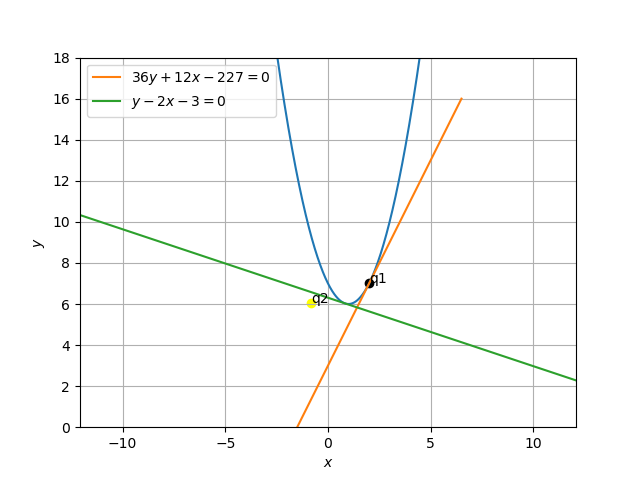
\includegraphics[width=0.75\columnwidth]{chapters/12/6/3/15/figs/conic.png}
		\caption{}
		\label{fig:12/6/3/15}
  	\end{figure}
The parameters of the given conic are
\begin{align}
\vec{V} =\myvec{
	1 & 0\\
	0 & 0
	},
    \vec{u}=-\myvec{
	1 \\
	\frac{1}{2}
	},
    f=7
    \end{align}
\begin{enumerate}
	\item In this case,  the normal vector
		\begin{align}\vec{n}_1 = \myvec{2 \\ -1}\end{align}
			Since 
$\vec{V}$ is not invertible,  
		%Then given the normal vector \begin{align}\vec{n}\end{align}\, 
	the point of contact is given by 
\eqref{eq:conic_tangent_q_eigen} resulting in 
		%the matrix equation
\begin{align}
\myvec{\myvec{-1 \\ -\frac{1}{2}} + \frac{1}{2}\myvec{2 \\ -1}^{\top} \vspace{0.3cm}\\ \myvec{
	1 & 0\\
	0 & 0\\
	}} \vec{q}_1 = \myvec{-7 \vspace{0.3cm}\\ \frac{1}{2}\myvec{2 \\ -1} - \myvec{-1 \\ -\frac{1}{2}}}
\end{align}
By solving the above equation, we can get the point of contact as
    \begin{align}
  \vec{q}_1=\myvec{
	2 \\
	7 \\
	}
\end{align}
The 
tangent equation is then obtained as
\begin{align}
      \vec{n}_1^{\top}(\vec{x}-\vec{q}_1) = 0
  \\
	\implies  \myvec{2 & -1}\vec{x}+3 = 0
\end{align}
\item 
In this case, 
		\begin{align}\vec{n}_2 = \myvec{1 \\ 3} \end{align}
resulting in 
\begin{align}
\myvec{\myvec{-1 \\ -\frac{1}{2}} + -\frac{1}{6}\myvec{1 \\ 3}^{\top} \vspace{0.3cm}\\ \myvec{
	1 & 0\\
	0 & 0\\
	}} \vec{q}_2 = \myvec{-7 \vspace{0.3cm}\\ -\frac{1}{6}\myvec{1 \\ 3} - \myvec{-1 \\ -\frac{1}{2}}}
\end{align}
    \begin{align}
	    \text{or, }  \vec{q}_2=\myvec{
	\frac{5}{6}
\\
	\frac{217}{36}
	}
\end{align}
The tangent equation is
\begin{align}
      \vec{n}_2^{\top}(\vec{x}-\vec{q}_2) = 0
      \\
	\text{or, }    \myvec{1 & 3}\vec{x}= \frac{227}{12}
\end{align}
\end{enumerate}
		See \figref{fig:12/6/3/15}.

\item Find the points on the curve $x^2+y^2-2x-3=0$ at which the tangents are parallel to the x-axis.
\label{chapters/12/6/3/19}
\\
\solution
Given that 
\begin{align}
	\vec{u} = \myvec{-1\\0},\,
	f = -3
\end{align}
Hence, the centre and radius are given as
\begin{align}
	\vec{c} = -\vec{u} = \myvec{1\\0},\,
	r = \sqrt{\norm{\vec{u}}^2 - f}
	  = 2
\end{align}
From \eqref{eq:conic_tangent_qk-circ},
the points of contact for the tangent are given by
\begin{align}
	\label{eq:chapters/12/6/3/19/eq3}
	\vec{q}_{ij} = \brak{\pm r\frac{\vec{n}_j}{\norm{\vec{n}_j}}-\vec{u}} \text{ i,j} = 1,2
\end{align}
Since, tangents are parallel to the x-axis, the normal is given as
\begin{align}
	\vec{n} = \myvec{0\\1}
\end{align}
Substituting in \eqref{eq:chapters/12/6/3/19/eq3} we get
\begin{align}
	\vec{q}_{11} &= \brak{\pm 2\myvec{0\\1} - \myvec{-1\\0}}\\
	&= \myvec{1\\-2},\myvec{1\\2}
\end{align}
Hence, the two points of contact are
\begin{align}
	\myvec{1\\2} \text{ and } \myvec{1\\-2}
\end{align}
See \figref{fig:chapters/12/6/3/19/Fig1}.
\begin{figure}[H]
	\begin{center} 
	    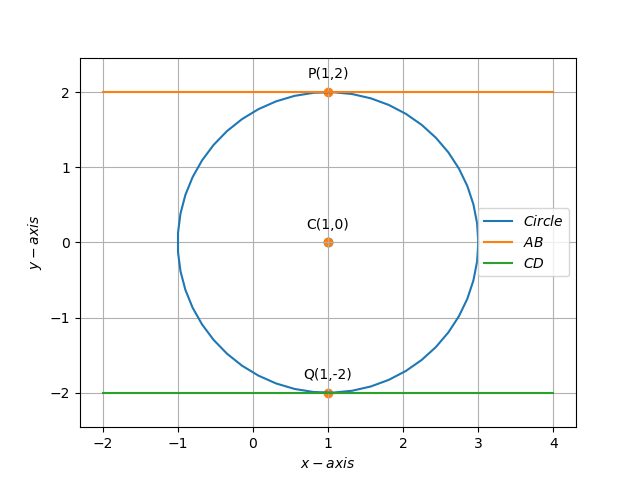
\includegraphics[width=0.75\columnwidth]{chapters/12/6/3/19/figs/tan1}
	\end{center}
\caption{}
\label{fig:chapters/12/6/3/19/Fig1}
\end{figure}






















\item 
Find the equation of the tangent to the curve 
\begin{align}
	y = \sqrt{3x-2}
\end{align}
which is parallel to the line
\begin{align}
	4x-2y+5 = 0
\end{align}
\solution 
\label{chapters/12/6/3/25}
\iffalse
\documentclass[journal,10pt,twocolumn]{article}
\usepackage{graphicx}
\usepackage[margin=0.5in]{geometry}
\usepackage[cmex10]{amsmath}
\usepackage{array}
\usepackage{booktabs}
\usepackage{mathtools}
\usepackage{multicol}
\usepackage[utf8]{inputenc}
\title{\textbf{Conic section Assignment}}
\author{T.Varsha Reddy}
\date{September 2022}


\providecommand{\norm}[1]{\left\lVert#1\right\rVert}
\providecommand{\abs}[1]{\left\vert#1\right\vert}
\let\vec\mathbf
\newcommand{\myvec}[1]{\ensuremath{\begin{pmatrix}#1\end{pmatrix}}}
\newcommand{\mydet}[1]{\ensuremath{\begin{vmatrix}#1\end{vmatrix}}}
\providecommand{\brak}[1]{\ensuremath{\left(#1\right)}}
\providecommand{\lbrak}[1]{\ensuremath{\left(#1\right.}}
\providecommand{\rbrak}[1]{\ensuremath{\left.#1\right)}}
\providecommand{\sbrak}[1]{\ensuremath{{}\left[#1\right]}}

\begin{document}

\maketitle
\section{Problem Statement}
\fi
Find the equation of the tangent to the curve 
\begin{align}
	y = \sqrt{3x-2}
\end{align}
which is parallel to the line
\begin{align}
	4x-2y+5 = 0
\end{align}
\solution 
\iffalse
\section{Solution}
The given equation of parabola $y^2 = 3x-2$ can be written in the general quadratic form as
\begin{align}
    \label{12/6/3/25eq:conic_quad_form}
    \vec{x}^{\top}\vec{V}\vec{x}+2\vec{u}^{\top}\vec{x}+f=0
    \end{align}
where
\fi
The parameters for the given conic are
\begin{align}
	\label{12/6/3/25eq:V_matrix}
	\vec{V} &= \myvec{0 & 0\\0 & 1},
	\\
	\label{12/6/3/25eq:u_vector}
	\vec{u} &= \myvec{-3/2\\0},
	\\
	\label{12/6/3/25eq:f_value}
	f &= 2
	%\\
\end{align}
which represent a parabola. 
Following the approach in problem 
\ref{chapters/12/6/3/15},
\iffalse
Thus can be expressed as by choosing
\begin{align}
%\label{12/6/3/25eq:eta}
Ki = \frac{\vec{Pi}^T\vec{u}}{\vec{Pi}^T\vec{n}}
\end{align}
%\begin{center}
   where
   \fi
   \begin{align}
     \vec{p_1} &= \myvec{1\\0},
     \\
     \vec{n} &= \myvec{-2\\1},
    \end{align}
    \iffalse
   
%\end{center}
If V is non invertible,given the normal vector $\eta$,the point of contact is given by the matrix equation. 

\begin{align}
    \myvec{( \vec{u}+\vec{ki}\vec{n})^T\\ \vec{V}}\vec{q} &= \myvec{-f \\ (\vec{Ki}\vec{n}-\vec{u})}  &\abs{V} &= 0
    \label{12/6/3/25eq:conic_parab_c}
    \end{align}
Substituting appropriate values from \eqref{12/6/3/25eq:V_matrix}, \eqref{12/6/3/25eq:u_vector}, \eqref{12/6/3/25eq:f_value}, and into \eqref{12/6/3/25eq:conic_parab_c}, the below matrix equation is obtained
\fi
yielding the matrix equation
\begin{align}
	\label{12/6/3/25eq:vertex_system}
	\myvec{-3&0\\0& 0\\0& 1}\vec{q} = \myvec{-41/16\\0 \\3/4}\\
\end{align}
The augmented matrix for \eqref{12/6/3/25eq:vertex_system} can be expressed as
\begin{align}
	%\label{12/6/3/25eq:vertex_solv1}
	%\myvec{-3&0&\vrule&2\\0&0&\vrule&0\\0&1&\vrule&0}\\ 	
	%\label{12/6/3/25eq:vertex_solv2}
	\xleftrightarrow[]{R_2 \leftrightarrow R_3}\myvec{-3&0&\vrule&-41/16\\0&1&\vrule&0\\0&0&\vrule&3/4}\\
	\label{12/6/3/25eq:vertex_solv3}
	\xleftrightarrow[]{-\frac{R_1}{-3} \leftarrow R_2}\myvec{1&0&\vrule&41/48\\0&1&\vrule&0\\0&0&\vrule&3/4}\\
	\label{12/6/3/25eq:vertex_solv4}
	\implies\vec{q} = \myvec{\frac{41}{48}\\\frac{3}{4}}
\end{align}
The equation of tangent is then obtained as
\begin{align}
	\myvec{-2 & 1}\vec{x} +\frac{23}{24} = 0 
\end{align}
See Fig. 
		\ref{fig:12/6/3/25}.
	\begin{figure}[!h]
		\centering
 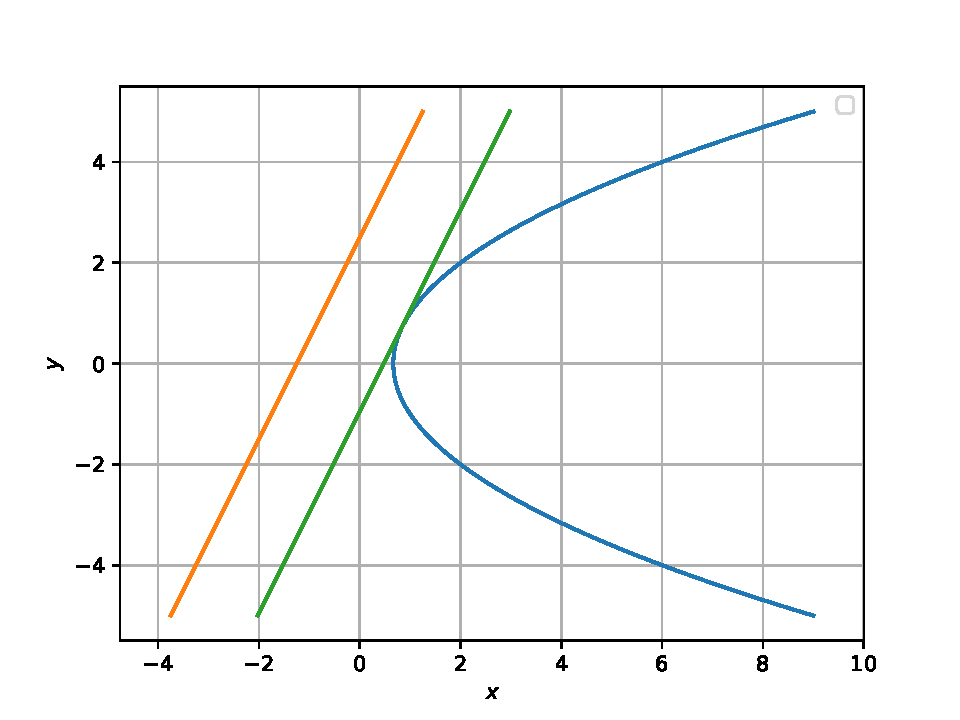
\includegraphics[width=\columnwidth]{chapters/12/6/3/25/figs/conic.pdf}
		\caption{}
		\label{fig:12/6/3/25}
  	\end{figure}
\iffalse
\begin{center}
\begin{align}
 \vec{(Vq+u)}^{\top}\vec{X}+\vec{u}^{\top}\vec{q}+\vec{f} =0 
\end{align}
\end{center}
\section{ Construction}
%\includegraphics[scale=0.5]{../Documents/co.pdf} 
%\includegraphics[scale=0.5]{co.pdf} 
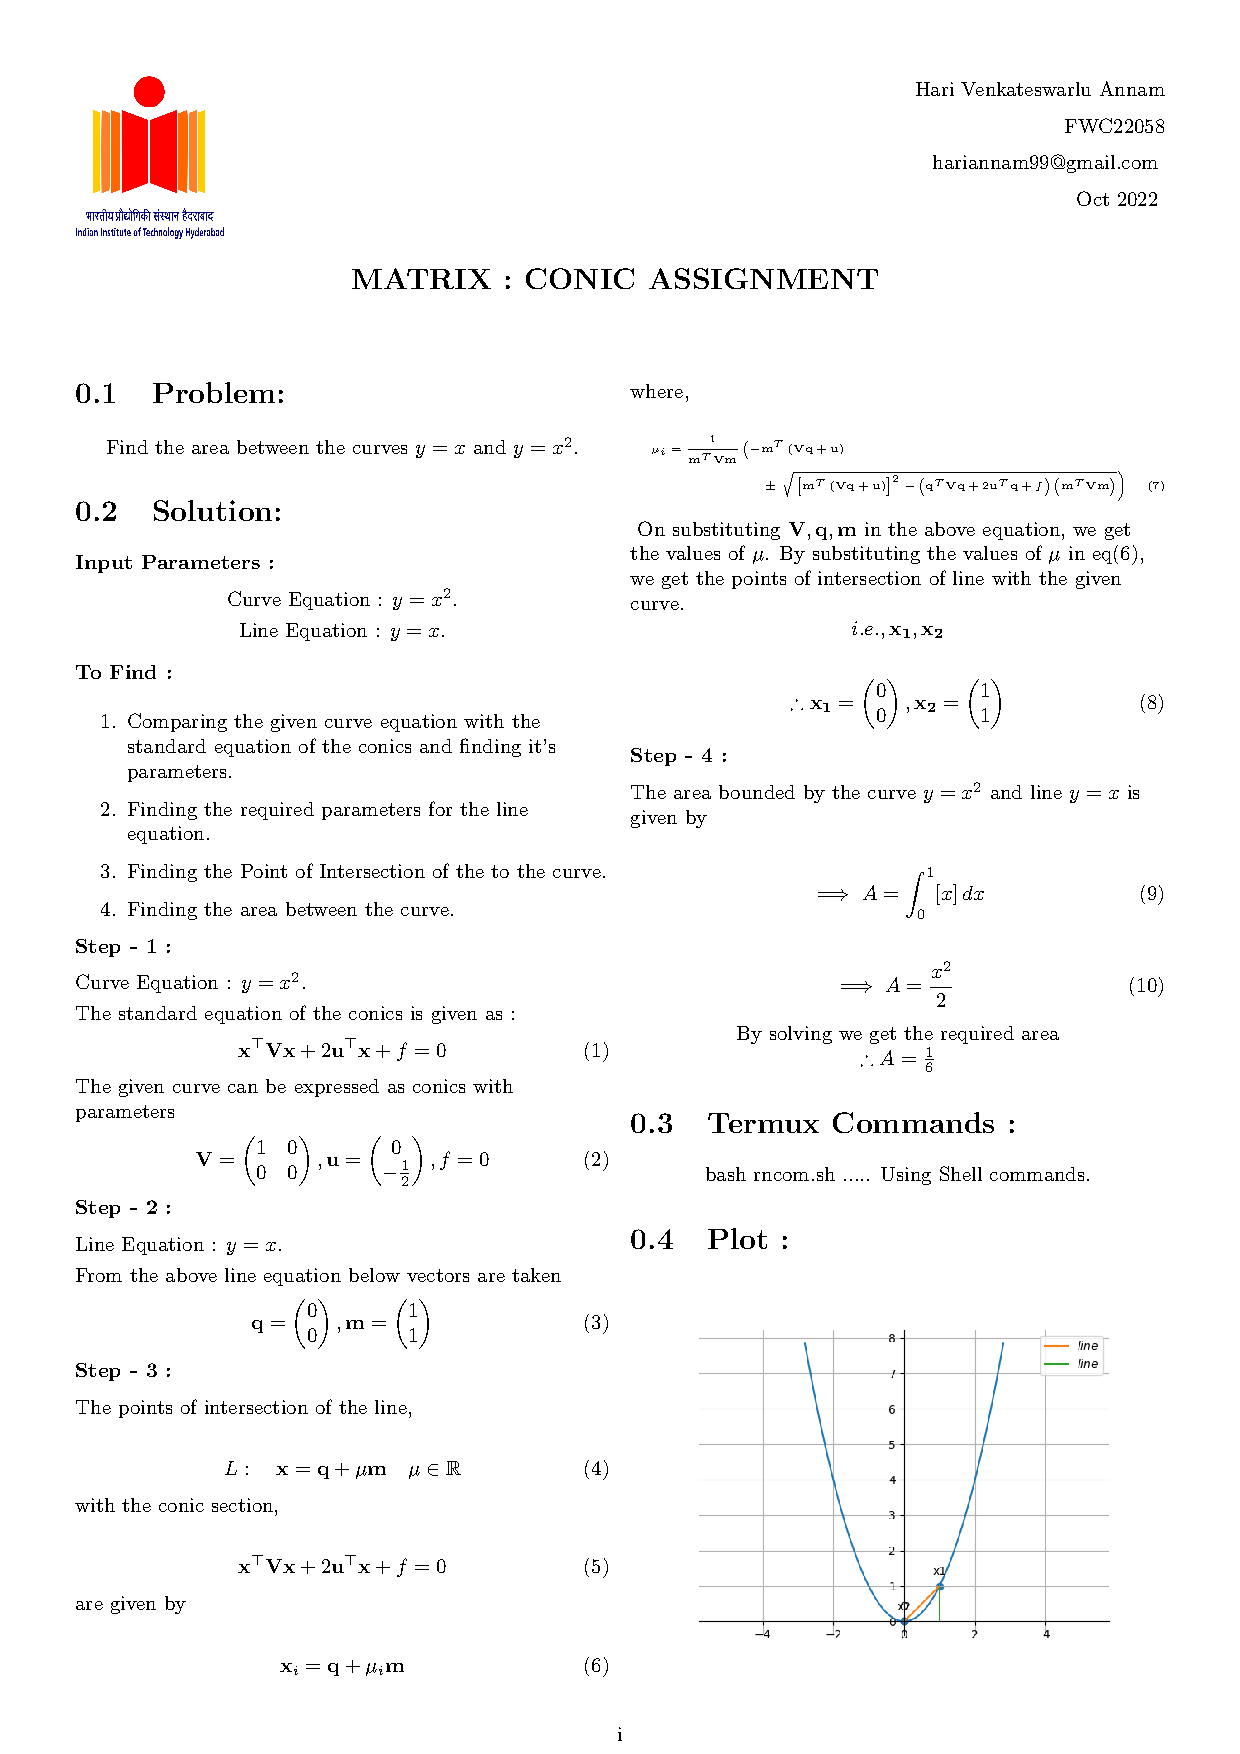
\includegraphics[scale=0.5]{conic.pdf} 
%\vspace{3mm}
%\url{https://github.com/9705701645/FWC/blob/main/co.py}
%\begin{multicols}
 %Download the code \\
%\href{https://github.com/9705701645/FWC/blob/main/co.py}{Assignment-5}.
%\end{multicols}
\end{document}


\fi

\item 
Find the point at which the line $y = x + 1$ is a tangent to the curve $y^2 = 4x$.
\\
\solution 
\label{chapters/12/6/3/27}
	\begin{figure}[H]
		\centering
 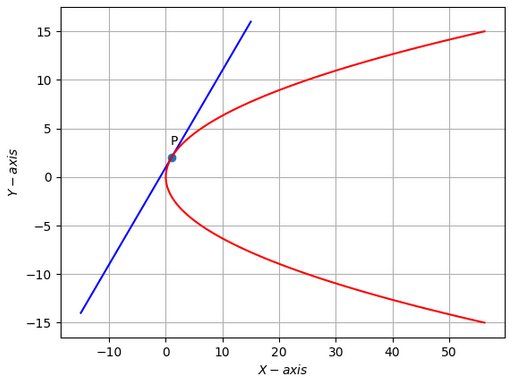
\includegraphics[width=0.75\columnwidth]{chapters/12/6/3/27/figs/conicfig.png}
		\caption{}
		\label{fig:12/6/3/27}
  	\end{figure}
The parameters of the conic are
\begin{align}
 \vec{V} = \myvec{0&0\\0&1},  \vec{u} = \myvec{-2&0}, f = 0 
\end{align}
Following the approach in Problem 
\ref{chapters/12/6/3/15},
since
\begin{align}
	\vec{n} = \myvec{1 \\ -1}
\end{align}
we obtain
\begin{align}
	\vec{q} = \myvec{1 \\ 2}
\end{align}
See 
		\figref{fig:12/6/3/27}.


    \item The point on the curve 
\label{chapters/12/6/5/27}
    \begin{align}
        x^2 = 2y
        \label{eq:chapters/12/6/5/27/curve}
    \end{align}
    which is nearest to the point 
    $\vec{P} = \myvec{0\\5}$ is
    \begin{enumerate}
        \item $\myvec{2\sqrt{2}\\4}$
        \item $\myvec{2\sqrt{2}\\0}$
        \item $\myvec{0\\0}$
        \item $\myvec{2\\2}$
    \end{enumerate}
    \solution 
		We rewrite the conic \eqref{eq:chapters/12/6/5/27/curve} in matrix form.
    \begin{align}
        \vec{x}^\top\myvec{1&0\\0&0}\vec{x} + 2\myvec{0&-1}\vec{x} = 0
        \label{eq:chapters/12/6/5/27/curve-mtx}
    \end{align}
    Comparing with the general equation of the conic,
    \begin{align}
        \vec{V}_0 = \myvec{1&0\\0&0},\
        \vec{u}_0 = \myvec{0\\-1},\ 
        f_0 = 0 
    \end{align}
    Therefore, the equation of the normal where $\vec{q}$ is the point of contact 
    and 
\begin{align}
    \vec{R} \triangleq \myvec{0&-1\\1&0} 
\end{align}
is
    \begin{align}
	    \brak{\vec{V}_0\vec{q}+\vec{u}_0}^\top\vec{R}\brak{\myvec{0\\5}-\vec{q}} &= 0
        \label{eq:chapters/12/6/5/27/normal}
    \end{align}
    Substituting appropriate values and simplifying, we get 
    \begin{align}
	    \vec{q}^\top\myvec{0&1\\0&0}\vec{q} + 2\myvec{-2 & 0}\vec{q}= 0
        \label{eq:chapters/12/6/5/27/q-eqn}
    \end{align}
    which can be expressed as 
    \begin{multline}
	    \frac{1}{2}\lcbrak{
		    \vec{q}^\top\myvec{0&1\\0&0}\vec{q} + 2\myvec{-2 & 0}\vec{q}}
	\\
	    +
	    \rcbrak{
		    \vec{q}^\top\myvec{0&1\\0&0}^\top\vec{q} + 2\myvec{-2 & 0}\vec{q}}= 0
    \end{multline}
    yielding
    \begin{align}
	    \vec{q}^\top\myvec{0&\frac{1}{2}\\\frac{1}{2}&0}\vec{q} + 2\myvec{-2 &0}\vec{q} = 0
        \label{eq:chapters/12/6/5/27/q-affine}
    \end{align}
        \eqref{eq:chapters/12/6/5/27/q-affine}
	also looks like a conic with parameters
    \begin{align}
        \vec{V} = \myvec{1&0\\0&0},\
        \vec{u} = \myvec{0\\-1},\ 
        f = 0 
    \end{align}
The eigenparameters of $\vec{V}$ are
    \begin{align}
        \label{eq:chapters/12/6/5/27/PD}
        \vec{P} = \myvec{1&1\\1&-1},\ \vec{D} = \myvec{1&0\\0&-1}
    \end{align}
    Applying the affine transformation
    \begin{align}
        \label{eq:chapters/12/6/5/27/affine}
        \vec{q} &= \vec{Py} + \vec{c} \\
        \vec{c} &= -\vec{V}^{-1}\vec{u} 
 =\myvec{0\\4} \\
        f_0 &= \vec{u}^\top\vec{V}^{-1}\vec{u} - f 
            =  0
    \end{align}
$\because \det{V} = -\frac{1}{4} \neq 0$, 
	  using \eqref{eq:pair-cond},
        \eqref{eq:chapters/12/6/5/27/q-affine}
 represents a pair of straight lines.
      From \eqref{eq:pair-conic},
        \eqref{eq:chapters/12/6/5/27/PD},
	\eqref{eq:incircle-disc-v}
	and 
	\eqref{eq:incircle-disc-v-lam},
    \begin{align}
%        y_1^2-y_2^2 &= 0 \\
%        \implies y_1 &= \pm y_2 \\
%        \implies \vec{y} &= \myvec{a\\\pm a},\ a \in \mathbb{R}
\vec{y} = \kappa\myvec{1\\\pm 1}.
        \label{eq:chapters/12/6/5/27/y-sol}
    \end{align}
    Hence, using 
        \eqref{eq:chapters/12/6/5/27/affine},
    \begin{align}
        \vec{q} 
                = \myvec{0\\4}+\kappa\myvec{1\\\pm 1},
%                &= \myvec{a\pm a\\a\mp a+4} \\
        \label{eq:chapters/12/6/5/27/x-case}
    \end{align}
which, upon substituting in 
        \eqref{eq:chapters/12/6/5/27/curve-mtx}
	and solving for $\kappa$ yields
\begin{align}
	\kappa = \pm \sqrt{2}, -2.
\end{align}
 Thus, the points of contact are
    \begin{align}
        \vec{q}  = \cbrak{\myvec{\pm 2\sqrt{2}\\4},\myvec{0\\0}}
        \label{eq:chapters/12/6/5/27/poc-ans}
    \end{align}
    The nearest point out of these three candidates for $\vec{q}$ is
    $\myvec{\pm2\sqrt{2}\\4}$. 
See \figref{fig:chapters/12/6/5/27/normal}.
\begin{figure}[!ht]
        \centering
        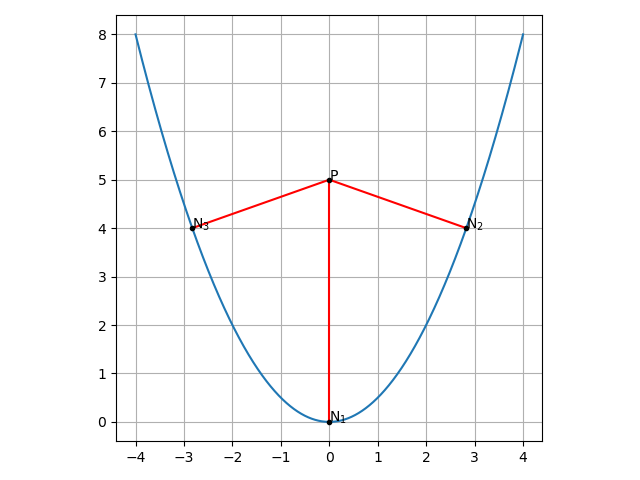
\includegraphics[width=\columnwidth]{chapters/12/6/5/27/figs/normal.png}
        \caption{}
        \label{fig:chapters/12/6/5/27/normal}
    \end{figure}

\item 
Find the equation of the normal to curve $x^2 = 4y$ which passes through the point
(1, 2).
\\
\solution 
\label{chapters/12/6/6/4}
	\begin{figure}[!h]
		\centering
 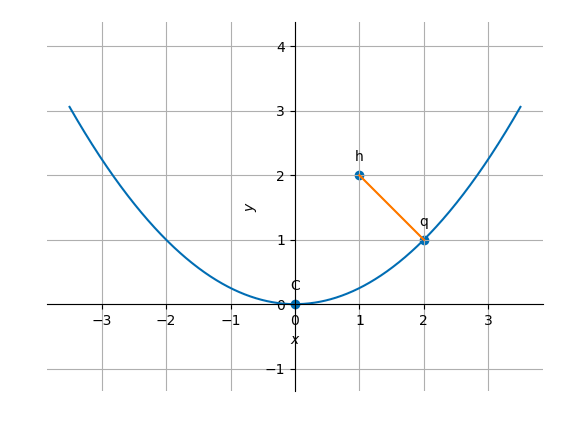
\includegraphics[width=\columnwidth]{chapters/12/6/6/4/figs/conics.png}
		\caption{}
		\label{fig:12/6/6/4}
  	\end{figure}
The conic parameters are
\begin{align}
	\vec{V} = \myvec{1 & 0\\0 & 0},
	\vec{u} = \myvec{0\\-2},
	f &= 0
	%\\
\end{align}
Choosing the direction and normal vectors as
\begin{align}
	\vec{m} = \myvec{1 \\ m}, \
	\vec{n} = \myvec{-m \\ 1}, 
\end{align}
and substituting these values in
	\eqref{eq:point_of_tangency-m},
% \eqref{eq:normal_solution}, 
 we obtain
\begin{align}
m = 1
\end{align}
as the only real solution.  Thus, 
\begin{align}
%\vec{n} = \myvec{1 \\ 1},
	\vec{m} = \myvec{1 \\ 1}, 
%    \mu = -1
\end{align}
and 
	the equation of the normal is then obtained as
\begin{align}
	\vec{m}^{\top}\brak{\vec{x}-\vec{h}} &= 0
	\\
	\implies
\myvec{
1 & 1
}
		\vec{x}
	&=
\myvec{
1 & 1
}
	\myvec{1 \\2 }
	\\
	&= 3
\end{align}
		See \figref{fig:12/6/6/4}.

\item 
 The line $y=mx+1$ is a tangent to the curve $y^2 = 4x$, find the value of $m$. 
 \\
 \solution 
\label{chapters/12/6/6/21}
	\begin{figure}[H]
		\centering
 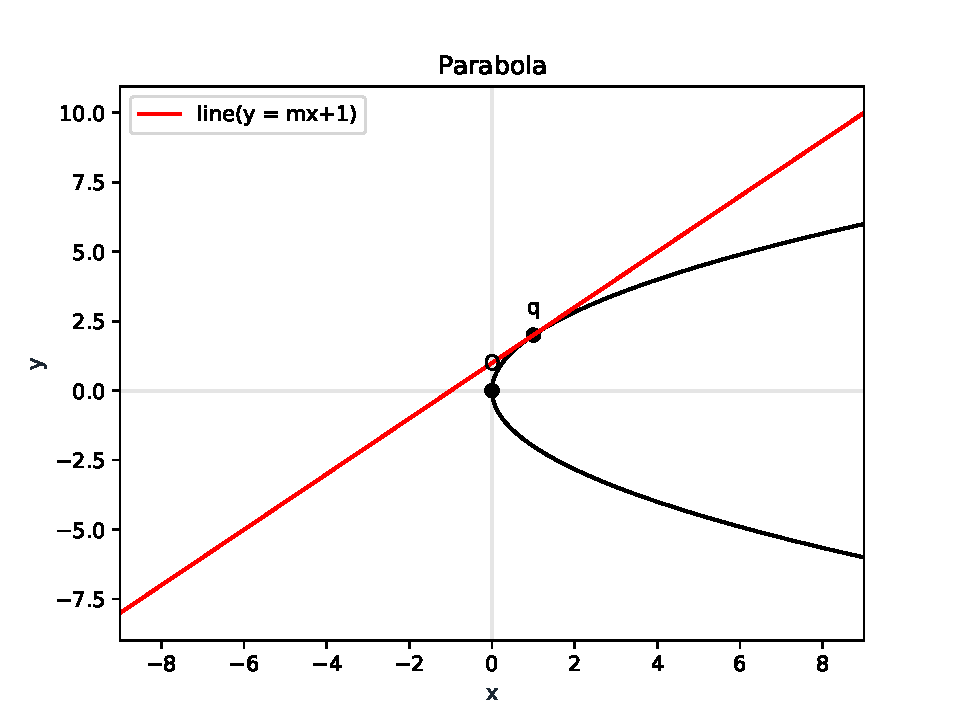
\includegraphics[width=0.75\columnwidth]{chapters/12/6/6/21/figs/im.pdf}
		\caption{}
		\label{fig:12/6/6/21}
  	\end{figure}
The parameters for the given conic are
\begin{align}
    \vec{V} = \myvec{0&0\\0&1}, \vec{u} = \myvec{-2\\0}, f = 0
		\label{eq:12/6/6/21/param}
\end{align}
The given tangent can be expressed in parametric form as
\begin{align}
		\label{eq:12/6/6/21/tangent}
\vec{x} = \vec{e}_2 + \mu\vec{m}
\end{align}
Substituting from 
		\eqref{eq:12/6/6/21/tangent}
		and
		\eqref{eq:12/6/6/21/param}
		in 
	  \eqref{eq:h-tangents-cond}
and solving, we obtain 
\begin{align}
	m = 1.
\end{align}
		See \figref{fig:12/6/6/21}.

\item 
\label{chapters/12/6/6/22}
Find the normal at the point (1,1) on the curve 
\begin{align}
2y+x^2=3
\end{align}
\solution
\iffalse
\documentclass[journal,10pt,twocolumn]{article}
\usepackage{graphicx, float}
\usepackage[margin=0.5in]{geometry}
\usepackage{amsmath, bm}
\usepackage{array}
\usepackage{booktabs}
\usepackage[utf8]{inputenc}
\usepackage{amsfonts}
\usepackage{amssymb}
\usepackage{graphicx}
\usepackage{multicol}
\usepackage{tabularx}
\usepackage{hyperref}
\usepackage{mathtools}
\DeclareUnicodeCharacter{2212}{-}
\providecommand{\norm}[1]{\left\lVert#1\right\rVert}
\providecommand{\abs}[1]{\left\vert#1\right\vert}
\let\vec\mathbf
\newcommand{\myvec}[1]{\ensuremath{\begin{pmatrix}#1\end{pmatrix}}}
\newcommand{\mydet}[1]{\ensuremath{\begin{vmatrix}#1\end{vmatrix}}}
\providecommand{\brak}[1]{\ensuremath{\left(#1\right)}}
\providecommand{\lbrak}[1]{\ensuremath{\left(#1\right.}}
\providecommand{\rbrak}[1]{\ensuremath{\left.#1\right)}}
\providecommand{\sbrak}[1]{\ensuremath{{}\left[#1\right]}}
%\providecommand{\norm}[1]{\left\lVert#1\right\rVert}
%\providecommand{\sbrak}[1]{\ensuremath{{}\left[#1\right]}}
%\providecommand{\lsbrak}[1]{\ensuremath{{}\left[#1\right.}}
%\providecommand{\rsbrak}[1]{\ensuremath{{}\left.#1\right]}}
%\providecommand{\brak}[1]{\ensuremath{\left(#1\right)}}
%\providecommand{\lbrak}[1]{\ensuremath{\left(#1\right.}}
%\providecommand{\rbrak}[1]{\ensuremath{\left.#1\right)}}
%\providecommand{\cbrak}[1]{\ensuremath{\left\{#1\right\}}}
%\providecommand{\lcbrak}[1]{\ensuremath{\left\{#1\right.}}
%\providecommand{\rcbrak}[1]{\ensuremath{\left.#1\right\}}}
%\newcommand{\myvec}[1]{\ensuremath{\begin{pmatrix}#1\end{pmatrix}}}
%\let\vec\mathbf

\title{\textbf{Conic Assignment}}
\author{Srinivas Dulla \hspace{9cm} FWC22041}
\date{September 2022}

\begin{document}

\maketitle
\paragraph{\textit{Problem Statement} -
\fi
Find the normal at the point (1,1) on the curve 
\begin{align}
2y+x^2=3
\end{align}
\solution
Use
  \eqref{eq:conic_tangent_mq}
  with 
\begin{align}
	\vec{m} = \myvec{1 \\m}
\end{align}
\iffalse
(a)x+y=0  \hspace{2cm} (b)x-y=0\\ 
(c)x+y+1=0 \hspace{2cm}  (d)x-y=1\\}

\section*{\large Solution}

\begin{figure}[H]
\centering
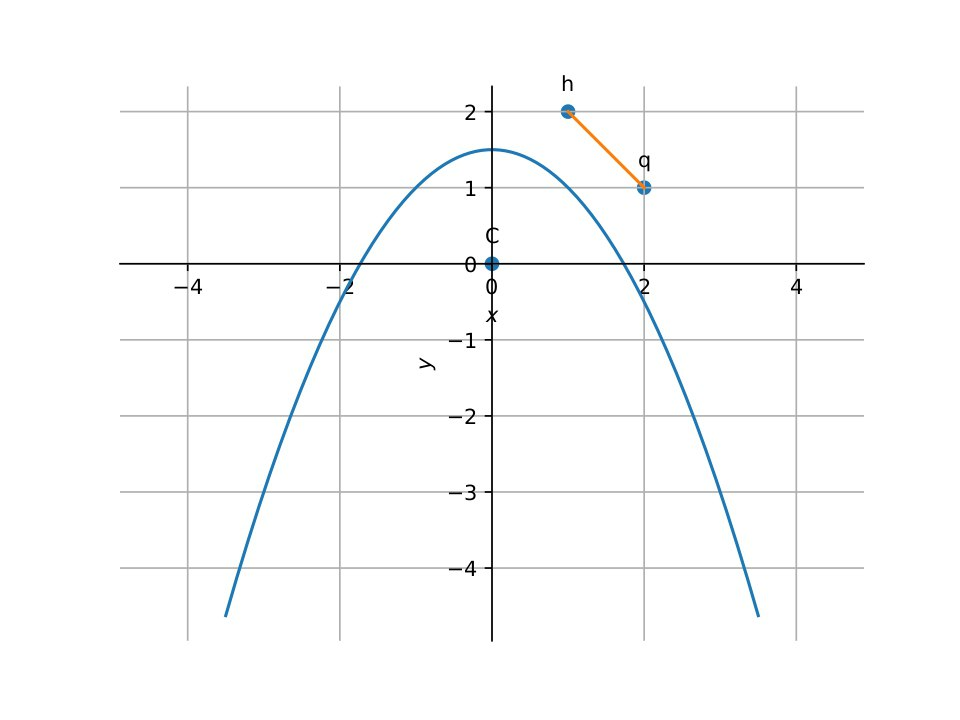
\includegraphics[width=1\columnwidth]{cone.jpg}
\caption{Tangents from A to circle through B, C and D}
\label{fig:triangle}
\end{figure}

The given equation of parabola $2y$+$x^2 = 3$ can be written in the general quadratic form as
\begin{align}
    \label{eq:conic_quad_form}
    \vec{x}^{\top}\vec{V}\vec{x}+2\vec{u}^{\top}\vec{x}+f=0
    \end{align}
where
\begin{align}
	\label{eq:V_matrix}
	\vec{V} &= \myvec{1 & 0\\0 & 0},
	\\
	\label{eq:u_vector}
	\vec{u} &= \myvec{0\\-2},
	\\
	\label{eq:f_value}
	f &= 3
	%\\
\end{align}

The parabola in (\ref{eq:conic_quad_form}) can be expressed in standard form (center/vertex at origin, major-axis - $x$ axis) as
\begin{align}
	\label{eq:conic_simp_parab}
	\vec{y}^{\top}\vec{D}\vec{y} &=  -2\eta\vec{e}_1^{\top}\vec{y}   & \abs{V} &= 0
\end{align}
 where
\begin{align}
	\label{eq:conic_affine}
	\vec{x} = \vec{P}\vec{y}+\vec{c} \quad \text{(Affine Transformation)}
\end{align}
\begin{align}
	\label{eq:conic_parmas_eig_def}
	\vec{P}^{\top}\vec{V}\vec{P} &= \vec{D}. \quad \text{(Eigenvalue Decomposition)}
	\\
	\label{eq:eigevalV}
	\vec{D} &= \myvec{\lambda_1 & 0\\ 0 & \lambda_2}, 
	\\
	\vec{P} &= \myvec{\vec{p}_1 & \vec{p}_2}, \quad \vec{P}^{\top}=\vec{P}^{-1},
	\label{eq:eigevecP}
	\\
	\label{eq:eta}
	\eta &=\vec{u}^{\top}\vec{p}_1
	\\
	\vec{e}_1 &=\myvec{1 \\ 0}
	\end{align}

To find $\vec{c}$ which is the center of the parabola in (\ref{eq:conic_quad_form}), substitute (\ref{eq:conic_affine}) in (\ref{eq:conic_quad_form})
\begin{multline}
\brak{\vec{P}\vec{y}+\vec{c}}^T\vec{V}\brak{\vec{P}\vec{y}+\vec{c}}+2\vec{u}^T\brak{\vec{P}\vec{y}+\vec{c}} + f = 0, 
\end{multline}
yielding 
\begin{multline}
\vec{y}^T\vec{P}^T\vec{V}\vec{P}\vec{y}+2\brak{\vec{V}\vec{c}+\vec{u}}^T\vec{P}\vec{y} +  \vec{c}^T\vec{V}\vec{c} 
\\
+2\vec{u}^T\vec{c} + f= 0
\label{eq:conic_simp_one}
\end{multline}
%
From \eqref{eq:conic_simp_one} and \eqref{eq:conic_parmas_eig_def},
\begin{multline}
\vec{y}^T\vec{D}\vec{y}+2\brak{\vec{V}\vec{c}+\vec{u}}^T\vec{P}\vec{y} +  \vec{c}^T\brak{\vec{V}\vec{c} + \vec{u}}
\\
+ \vec{u}^T\vec{c} + f= 0
\label{eq:conic_simp}
\end{multline}
For a parabola $\abs{\vec{V}} = 0, \lambda_1 = 0$ and
\begin{align}
\vec{V}\vec{p}_1 = 0, 
\vec{V}\vec{p}_2 = \lambda_2\vec{p}_2.
\label{eq:conic_parab_eig_prop} 
\end{align}
where $\vec{p}_1,\vec{p}_2$ are the eigenvectors of $\vec{V}$ such that  \eqref{eq:conic_parmas_eig_def}
%
\begin{align}
\vec{P} = \myvec{\vec{p}_1 & \vec{p}_2},
\label{eq:eig_matrix}
\end{align}
Substituting \eqref{eq:eig_matrix}
in \eqref{eq:conic_simp},
\begin{multline}
	\vec{y}^T\vec{D}\vec{y}+2\brak{\vec{c}^T\vec{V}+\vec{u}^T}\myvec{\vec{p}_1 & \vec{p}_2}\vec{y}
\\
+  \vec{c}^T\brak{\vec{V}\vec{c} + \vec{u}}+ \vec{u}^T\vec{c} + f= 0
\\
\implies \vec{y}^T\vec{D}\vec{y}
\\
+2\myvec{\brak{\vec{c}^T\vec{V}+\vec{u}^T}\vec{p}_1  \brak{\vec{c}^T\vec{V}+\vec{u}^T}\vec{p}_2}\vec{y}
\\
+  \vec{c}^T\brak{\vec{V}\vec{c} + \vec{u}}+ \vec{u}^T\vec{c} + f= 0
\\
\implies \vec{y}^T\vec{D}\vec{y}
\\
+2\myvec{\vec{u}^T\vec{p}_1 & \brak{\lambda_2\vec{c}^T+\vec{u}^T}\vec{p}_2}\vec{y}
\\
+  \vec{c}^T\brak{\vec{V}\vec{c} + \vec{u}}+ \vec{u}^T\vec{c} + f= 0
\text{ from } \eqref{eq:conic_parab_eig_prop}     \nonumber \\
\\
\implies \lambda_2y_2^2+2\brak{\vec{u}^T\vec{p}_1}y_1+  2y_2\brak{\lambda_2\vec{c}+\vec{u}}^T\vec{p}_2
\\
+  \vec{c}^T\brak{\vec{V}\vec{c} + \vec{u}}+ \vec{u}^T\vec{c} + f= 0
\label{eq:conic_parab_foc_len_temp} 
\end{multline}
which is the equation of a parabola. 
Thus, \eqref{eq:conic_parab_foc_len_temp} 
can be expressed as \eqref{eq:conic_simp_parab} by choosing
\begin{align}
%\label{eq:eta}
\eta = \vec{u}^T\vec{p}_1
\end{align}
and $\vec{c}$ in \eqref{eq:conic_simp} such that
\begin{align}
\label{eq:conic_parab_one}
\vec{P}^{T}\brak{\vec{V}\vec{c}+\vec{u}} &= \eta\myvec{1\\0}
\\
\vec{c}^T\brak{\vec{V}\vec{c} + \vec{u}}+ \vec{u}^T\vec{c} + f&= 0
\label{eq:conic_parab_two}
\end{align}
Multiplying \eqref{eq:conic_parab_one} by $\vec{P}$ yields
\begin{align}
\label{eq:conic_parab_one_eig}
\brak{\vec{V}\vec{c}+\vec{u}} &= \eta\vec{p}_1,
\end{align}
which, upon substituting in \eqref{eq:conic_parab_two}
results in 
\begin{align}
\eta\vec{c}^T\vec{p}_1 + \vec{u}^T\vec{c} + f&= 0
\label{eq:conic_parab_two_eig}
\end{align}
\eqref{eq:conic_parab_one_eig} and \eqref{eq:conic_parab_two_eig} can be clubbed together to obtain \eqref{eq:conic_parab_c}.
\begin{align}
    \myvec{ \vec{u}^{\top}+\eta\vec{p}_1^{\top} \\ \vec{V}}\vec{c} &= \myvec{-f \\ \eta\vec{p}_1-\vec{u}}  &\abs{V} &= 0
    \label{eq:conic_parab_c}
    \end{align}
Substituting appropriate values from \eqref{eq:V_matrix}, \eqref{eq:u_vector}, \eqref{eq:f_value}, \eqref{eq:eigevecP}, and \eqref{eq:eta} into \eqref{eq:conic_parab_c}, the below matrix equation is obtained
\begin{align}
	\label{eq:vertex_system}
	\myvec{0&-4\\1& 0\\0& 0}\vec{c} = \myvec{0 \\0 \\0}\\
\end{align}
The augmented matrix for \eqref{eq:vertex_system} can be expressed as
\begin{align}
	\label{eq:vertex_solv1}
	\myvec{0&-4&\vrule&0\\1&0&\vrule&0\\0&0&\vrule&0}\\ 	
	\label{eq:vertex_solv2}
	\xleftrightarrow[]{R_1 \leftrightarrow R_2}\myvec{1&0&\vrule&0\\0&-4&\vrule&0\\0&0&\vrule&0}\\
	\label{eq:vertex_solv3}
	\xleftrightarrow[]{-\frac{R_2}{4} \leftarrow R_2}\myvec{1&0&\vrule&0\\0&1&\vrule&0\\0&0&\vrule&0}\\
	\label{eq:vertex_solv4}
	\implies\vec{c} = \myvec{0\\0}
\end{align}

Let the point from which normals are drawn be $\vec{h}$. Then, the equation of the normal can be written as
\begin{align}
	\vec{x} = \vec{h} + \lambda\vec{m}
	\label{eq:normal_chord}
\end{align}
Say the point of intersection of \eqref{eq:normal_chord} with the conic is $\vec{q}$. A tangent drawn at $\vec{q}$ satisfies the equation
\begin{align}
	\label{eq:tangency_condition}
	\vec{n}^\top(\vec{Vq}+\vec{u}) = 0
\end{align}
Where $\vec{n}$ is the direction vector of the tangent and is perpendicular to $\vec{m}$ in \eqref{eq:normal_chord}.\\\\
In general, the parameter values for points of intersection of a line given by \eqref{eq:normal_chord} with a conic is given by
{\tiny
\begin{multline}
\lambda_i = \frac{1}
{
\vec{m}^T\vec{V}\vec{m}
}
\lbrak{-\vec{m}^T\brak{\vec{V}\vec{h}+\vec{u}}}
\\
\pm
\rbrak{\sqrt{
\sbrak{
\vec{m}^T\brak{\vec{V}\vec{h}+\vec{u}}
}^2
-
\brak
{
\vec{h}^T\vec{V}\vec{h} + 2\vec{u}^T\vec{h} +f
}
\brak{\vec{m}^T\vec{V}\vec{m}}
}
}
\label{eq:tangent_roots}
\end{multline}
}
Using \eqref{eq:tangent_roots} and \eqref{eq:normal_chord}, the intersection point $\vec{q}$ can be written as
\begin{align}
	\label{eq:point_of_tangency}
	\vec{q} = \vec{h} + \lambda_i\vec{m}
\end{align}
Substituting \eqref{eq:point_of_tangency} in \eqref{eq:tangency_condition},
\begin{align}
	\label{eq:normal_simp_1}
	\vec{n}^\top(\vec{V}(\vec{h}+\lambda_i\vec{m})+\vec{u}) = 0\\
	\label{eq:normal_simp_2}
	\implies \lambda_i\vec{n}^\top\vec{V}\vec{m} = -\vec{n}^\top(\vec{Vh}+\vec{u})
\end{align}
Substituting value of $\lambda_i$ from \eqref{eq:tangent_roots} in \eqref{eq:normal_simp_2}
{\tiny
\begin{multline}
	\frac{1}{\vec{m}^\top\vec{V}\vec{m}}\lbrak{-\vec{m}^\top\brak{\vec{Vh}+\vec{u}}} \\ 
	\pm \rbrak{\sqrt{\sbrak{\vec{m}^T\brak{\vec{V}\vec{h}+\vec{u}}}^2-\brak{\vec{h}^T\vec{V}\vec{h} + 2\vec{u}^T\vec{h} +f}\brak{\vec{m}^T\vec{V}\vec{m}}}}\vec{n}^\top\vec{V}\vec{m} \\
	= -\vec{n}^\top\brak{\vec{Vh}+\vec{u}}
	\label{eq:normal_simp_3}
\end{multline}
}
Rearranging the terms,
{\tiny
\begin{multline}
	\pm \sqrt{\sbrak{\vec{m}^T\brak{\vec{V}\vec{h}+\vec{u}}}^2-\brak{\vec{h}^T\vec{V}\vec{h} + 2\vec{u}^T\vec{h} +f}\brak{\vec{m}^T\vec{V}\vec{m}}} \brak{\vec{n}^\top\vec{V}\vec{m}} \\ = \brak{\vec{Vh}+\vec{u}}^\top\brak{\brak{\vec{n}^\top\vec{V}\vec{m}}\vec{m}-\brak{\vec{m}^\top\vec{V}\vec{m}}\vec{n}}
\end{multline}
}
Squaring on both sides
{\tiny
\begin{multline}
	\sbrak{\sbrak{\vec{m}^T\brak{\vec{V}\vec{h}+\vec{u}}}^2-\brak{\vec{h}^T\vec{V}\vec{h} + 2\vec{u}^T\vec{h} +f}\brak{\vec{m}^T\vec{V}\vec{m}}}\brak{\vec{n}^\top\vec{V}\vec{m}}^2 \\ = \sbrak{\brak{\vec{Vh}+\vec{u}}^\top\brak{\brak{\vec{n}^\top\vec{V}\vec{m}}\vec{m}-\brak{\vec{m}^\top\vec{V}\vec{m}}\vec{n}}}^2
	\label{eq:normal_solution}
\end{multline}
}\\
If $\vec{n}$ is taken as $\myvec{-\mu \\ 1}$, then $\vec{m}$ is $\myvec{-1 \\ -\mu}$. Substituting these values in \eqref{eq:normal_solution} and solving for $\mu$, the different possible normals passing through $\vec{h}$ are obtained.\\\\
Thus after solving we get the following values for $\mu$ = {-1, 1/2 - sqrt(3)*I/2, 1/2 + sqrt(3)*I/2}\\\\
Taking $\mu$=1 we get,
\begin{center}
$\vec{n} = \myvec{1 \\ 1}$, $\vec{m} = \myvec{-1 \\ 1}$\\
\end{center}
By calculating $\lambda_i$ from \eqref{eq:normal_simp_2}, we get
\begin{center}
    $\lambda_i = -1$
\end{center}
We find out $\vec{q}$ from \eqref{eq:point_of_tangency},
\begin{center}
where $\vec{h} = \myvec{1 \\ 2}$, $\vec{m} = \myvec{-1 \\ 1}$, $\lambda_i = -1$
\end{center}
\begin{center}
    $\vec{q} = \myvec{1 \\ 2} + (-1)\myvec{-1 \\ 1} = $\myvec{2 \\ 1}
\end{center}
\begin{center}
    Thus $\vec{q}$ satisfies Option(a) i.e. $x+y=3$
\end{center} 

\section*{\large Construction}
{
\setlength\extrarowheight{5pt}
\begin{tabular}{|c|c|c|}
	\hline
	\textbf{Symbol}&\textbf{Value}&\textbf{Description}\\[5pt]
	\hline
	$\vec{h}$&$\myvec{1 \\ 2}$&Given point through which Normal is passing\\[5pt]
	\hline
	$\vec{q}$&$\myvec{2 \\ 1}$&Foot of Normal\\[5pt]
	\hline
	$\vec{m}$ & $\myvec{-1 \\ 1}$ & Direction Vector of Normal\\[5pt]
	\hline
	$\vec{n}$ & $\myvec{1 \\ 1}$ & Direction Vector of Tangent at $\myvec{q}$\\
	\hline
	$\vec{P}$&\myvec{0&1\\1&0}&eigenvectors of $\vec{V}$\\[5pt]
	\hline
\end{tabular}
}

\end{document}
\fi

\end{enumerate}
